\documentclass[12pt, a4paper, oneside]{book}
\usepackage[margin=2cm]{geometry}
\usepackage[english]{babel}
\usepackage{amsmath}
\usepackage[T1]{fontenc}
\usepackage[utf8x]{inputenc}
\usepackage{graphicx}
\usepackage{listings}
\usepackage{hyperref}
\usepackage{framed}

\begin{document}
\title{\Huge{Mobile Collaboration Platform}\\\Large{documentation}}
\maketitle
\tableofcontents


\chapter{Description}

The Mobile Application Platform is a framework to share contents between applications on different near Android devices, such as phones or tablets. Using the framework an application can easily ask other unknown devices for the contents it needs.
The framework handles the discovering of other near devices and the connection with them to exchange queries or files.
The framework is provided as an installable APK file for ARMv6 and ARMv7 Android phones and tablets. These devices must have root permissions, needed to perform some operation such as enabling ad-hoc mode WiFi.

\begin{figure}[h!]
\centering
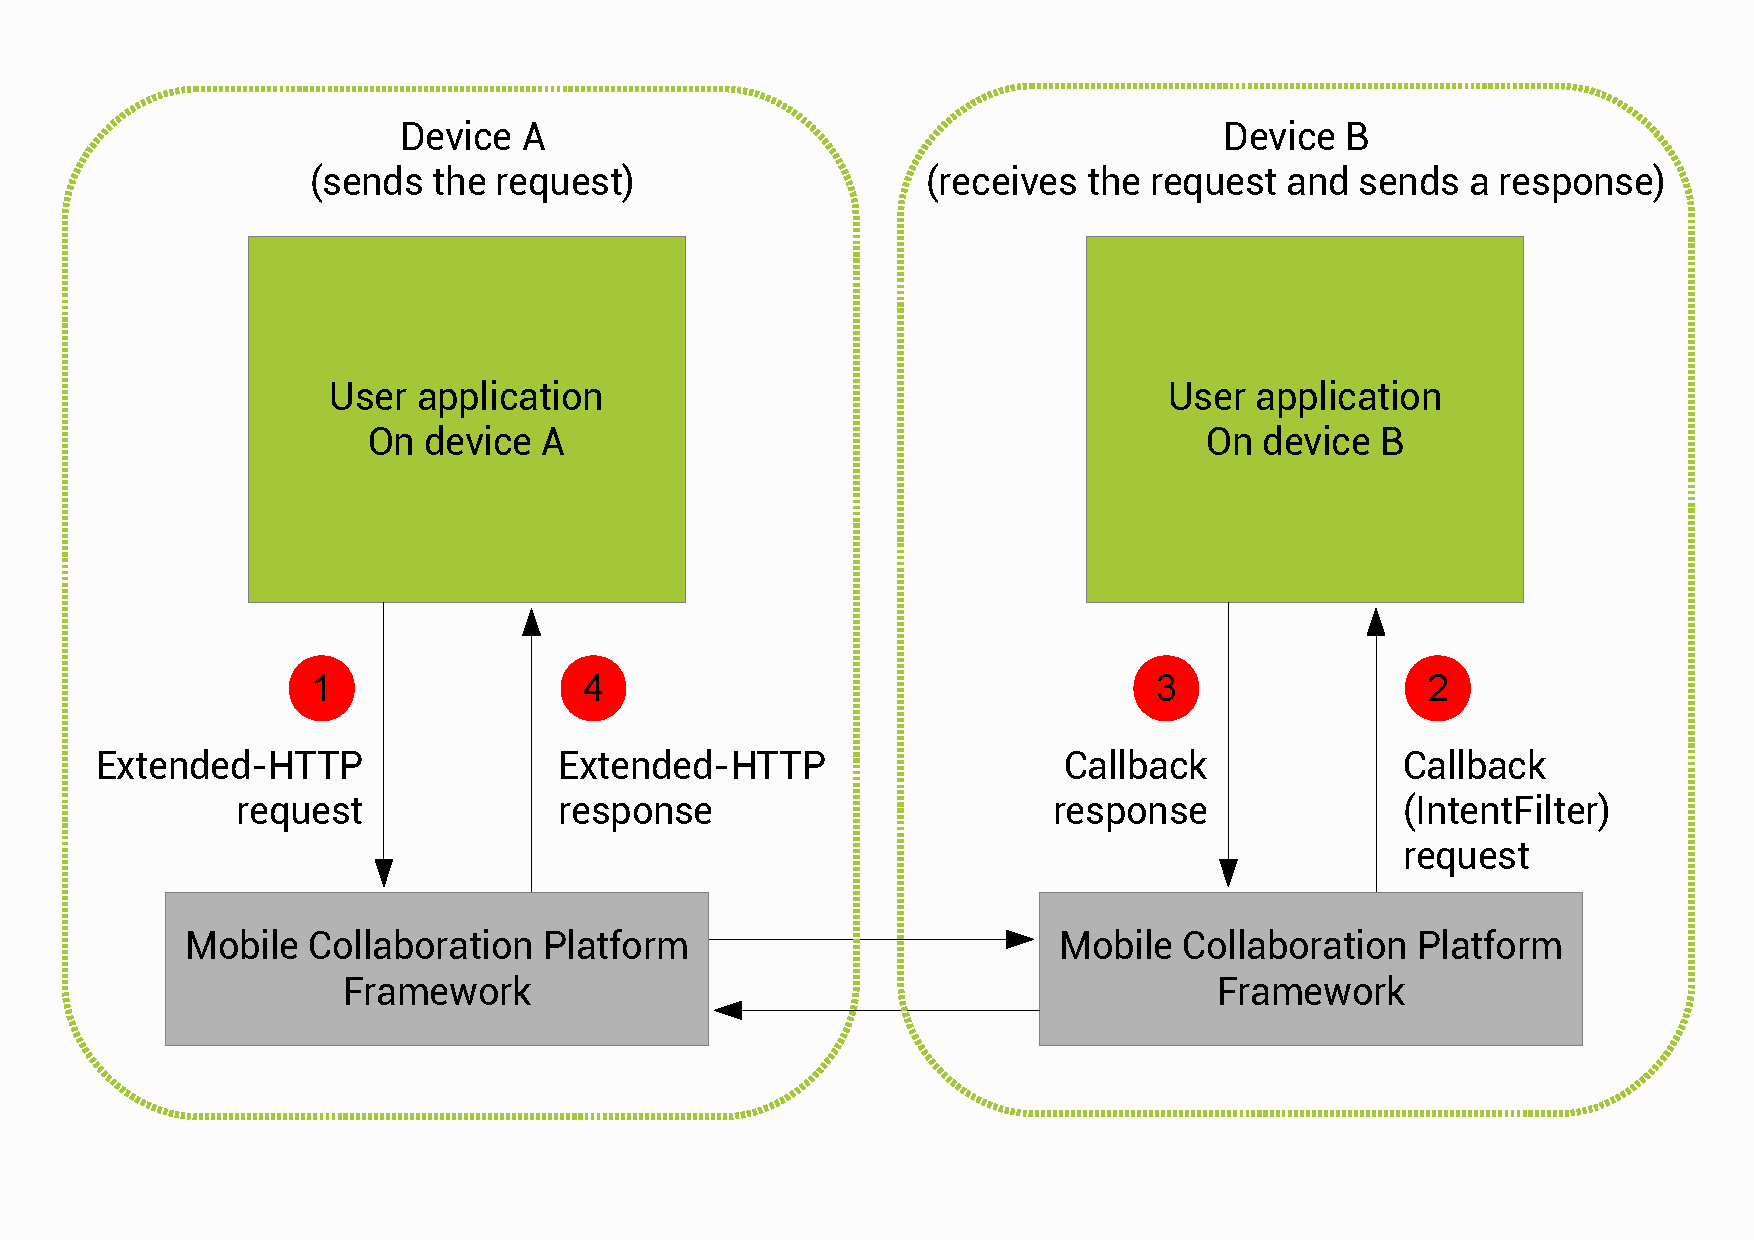
\includegraphics[scale=0.6]{images/SchemaFrameworkAltoLivello.pdf}
\caption{Message exchange for a query request/response}
\label{fig:platformSchemeQueryRequestResponse}
\end{figure}

\chapter{Framework usage}
To use the framework the user must first install and enable it. On the main interface (figure \ref{fig:platformActivity}) there are some options which can be set.

\begin{figure}[h!]
\centering
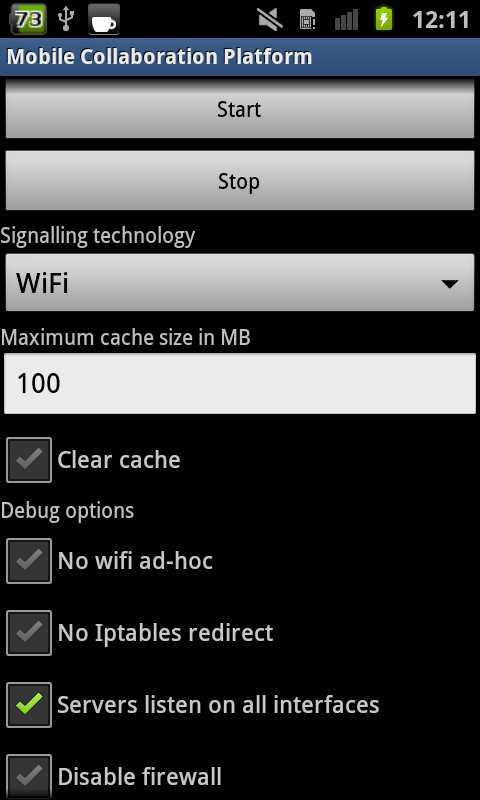
\includegraphics[scale=0.3]{images/platformActivity.png}
\caption{The platform main interface}
\label{fig:platformActivity}
\end{figure}

\begin{itemize}
\item \textbf{Signalling technology}: lets the user choose the technology to use for the signalling exchange. At the moment Wifi or Zigbee can be used;
\item \textbf{Maximum cache size}: lets the user choose the maximum amount of storage for the platform internal cache;
\item \textbf{Clear cache}: clears the platform internal cache;
\item \textbf{No wifi ad-hoc}: doesn't enable ad-hoc mode WiFi, so that the device can be used connected to a WiFi access point;
\item \textbf{No Iptables redirect}: doesn't enable the redirect of the HTTP traffic from the port 80 to the port 8080 (the redirect is only necessary for legacy apps);
\item \textbf{Servers listen on all interfaces}: internal framework servers listen also on 3G interface (this should be only enabled for debugging reasons);
\item \textbf{Disable firewall}: doesn't enable the builtin firewall (this should be only enabled for debugging reasons).
\end{itemize}

\chapter{Collaborative video downloading}
The framework can act as a proxy to download video files from an HTTP server. Before downloading these files from a 3G connections, the application searches if they are available on nearby devices running the same platform. In this case the download is performed locally.

The framework accepts normal HTTP requests and is completely transparent to legacy applications. For example it can be directly used with the Android default video player.

When the player sends an HTTP request for a video, it is intercepted by the proxy, which searches for nearby devices which have this file in cache. If no device is found, the file is downloaded from a 3G connection (if available) and it is stored in the local cache for future uses. At the moment this works only with the Apple's \textit{HTTP Live Streaming protocol}, which is based on a plain text playlist (.m3u8 files) and one or more \textit{MPEG transport stream} chunks (.ts files). More information about this protocol can be found here: \href{https://developer.apple.com/resources/http-streaming/}{https://developer.apple.com/resources/http-streaming/}

\chapter{Query-based content sharing}
Applications can use the framework to share contents with other mobile devices nearby. They can send queries and obtain answers or ask for certain files whose MD5 digest is already known (for example it was contained in the query response).
The interaction with the framework is done with simple Extended-HTTP messages. The framework listens for them on the local port 8080.

\section{Requests with query}
Requests containing queries are of the following form:
\begin{verbatim}
GET //MCP/QUERY HTTP/1.1
x-mcp-query: myquery
x-mcp-app: it.uniroma2.myApp
x-mcp-ttl: 10
\end{verbatim}
Requests MUST begin with \texttt{GET //MCP/QUERY HTTP/1.1}. The field \texttt{x-mcp-query} MUST contain the query, which MUST be a plain text string. The field \texttt{x-mcp-app}, instead, MUST contain the name of the application which is sending the request. This is important because this value is used from the devices which receive the request to choose the application to forward the message to. The optional field \texttt{x-mcp-ttl} CAN contain the time (in seconds) the framework waits for answers.
Received the request, the framework forwards the query broadcast to all the devices nearby and waits for their answers. These are immediately sent back to the application in response to the HTTP request.
The structure of the response messages is the following:
\begin{verbatim}
HTTP/1.1 200 OK
Connection: Keep-Alive
Transfer-Encoding: chunked
Content-Type: text/plain

[QUERY RESPONSE]
\end{verbatim}
Multiple answers can arrive for a single request because there may be several devices nearby who have the desired content.

\newpage
\begin{framed}
\textbf{IMPORTANT}: Query string MUST NOT contain the following symbols:
\begin{itemize}
\item <CR> \textit{ (Carriage return, \texttt{\textbackslash r} in Java)}
\item <LF> \textit{ (Line feed, \texttt{\textbackslash n} in Java)}
\item \texttt{;;} \textit{ (Two semicolons)}
\end{itemize}
\end{framed}

\begin{framed}
\textbf{IMPORTANT}: Responses to queries MUST contain a delimiter character! See the provided demo app for a usage example.
\end{framed}

\newpage
\section{Requests for files}
To request a certain file whose MD5 digest is already known, the structure of the request is the following:
\begin{verbatim}
GET //MCP/FILE HTTP/1.1
x-mcp-digest: abcdefghilmnopqrstuvz
x-mcp-app: it.uniroma2.myApp
\end{verbatim}
The field \texttt{x-mcp-digest} MUST contain the MD5 checksum of the file, while the field \texttt{x-mcp-app} MUST contain, as in the case of query requests, the name of the application which sent the request.
The structure of the responses is the following:
\begin{verbatim}
HTTP/1.1 200 OK
Content-type: [file mime type]
Content-length: [file length]

[FILE CONTENT]
\end{verbatim}
Unlike the requests with queries, in this case only one HTTP response is sent back containing the file, also if it is available on different devices. If the file is not found, a \textit{404 NOT FOUND} error is sent back.

\section{Interfaces to be implemented in applications}
To allow the proxy to interact with the application when a request from another device arrives, it is necessary to implement, in a Service, the following interface (which MUST be defined in the file \textit{it/uniroma2/mobilecollaborationplatform/querymanager/QueryManagerOp.aidl}):
\begin{verbatim}
package it.uniroma2.mobilecollaborationplatform.querymanager;

interface QueryManagerOp {
	String getQueryResponse(String query);
	String getFile(String digest);
}
\end{verbatim}

Here is an example of the Service and the content of the AndroidManifest file:
\lstset{language=Java, tabsize=2, basicstyle=\footnotesize , breaklines=true}
\lstinputlisting[title={QueryManager.java}]{QueryManager.java}
\lstset{language=XML, tabsize=2, basicstyle=\footnotesize , breaklines=true}
\lstinputlisting[title={AndroidManifest.xml}]{AndroidManifest.xml}
The intent filter is necessary for the framework to detect the presence of the application.

\chapter{Demo application}
Together with this document is provided a demo application which uses this framework. Refer to the code comments for details.
\end{document}